\documentclass{standalone}
\usepackage{pgf,tikz}
% Changing the definition of underbar in the kernel to allow for math mode
\makeatletter
	\def\munderbar#1{\underline{\sbox\tw@{$#1$}\dp\tw@\z@\box\tw@}}
\makeatother

\usetikzlibrary{positioning}

\begin{document}

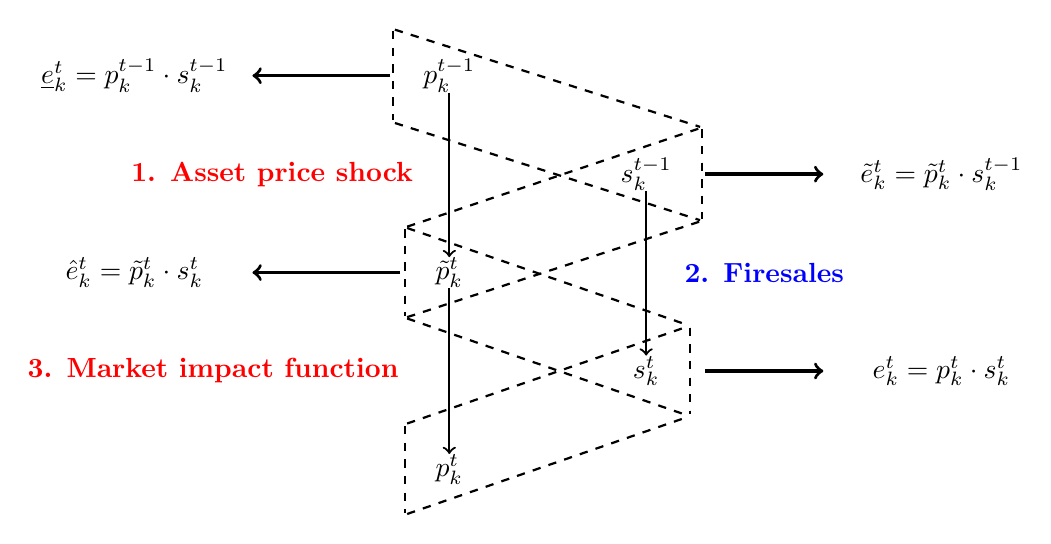
\begin{tikzpicture}
   [scale=0.5,every node/.style={draw=none,inner sep = 0pt}]
   
\node[](p1) at (0,10) {$p_{k}^{t-1}$};
\node[](p2) at (0,5) {$\tilde{p}_{k}^{t}$};
\node[](p3) at (0,0) {$p_{k}^{t}$};

\node[](s1) at (5,7.5) {$s_{k}^{t-1}$};
\node[](s2) at (5,2.5) {$s_{k}^{t}$};

%%%%%%%%%%%%%%%%%%%%%%%%%%%%%%%%%%%%%%%%%%%%%%%%%%%%%%%%%%%%%%%
% Box 1 = p_{k}^{t-1} x s_{k}^{t-1}
%%%%%%%%%%%%%%%%%%%%%%%%%%%%%%%%%%%%%%%%%%%%%%%%%%%%%%%%%%%%%%%

% Dashed box
\node[above left = 0.5cm of p1] (box1_TL) {};
\node[below left = 0.5cm of p1] (box1_BL) {};
\node[above right = 0.5cm of s1] (box1_TR) {};
\node[below right = 0.5cm of s1] (box1_BR) {};
	\draw[dashed, thick] (box1_TL) -- (box1_BL);
	\draw[dashed, thick] (box1_TR) -- (box1_BR);
	\draw[dashed, thick] (box1_BL) -- (box1_BR);
	\draw[dashed, thick] (box1_TL) -- (box1_TR);
	
% Portfolio value calculation
\draw[very thick,->] (-1.5,10) -- (-5,10);
\node[align = center] (p1s1) at (-8,10) {$\munderbar{e}_{k}^{t} =  p_{k}^{t-1}\cdot s_{k}^{t-1} $};

%%%%%%%%%%%%%%%%%%%%%%%%%%%%%%%%%%%%%%%%%%%%%%%%%%%%%%%%%%%%%%%
%Box 2 = \tilde{p}_{k}^{t} x s_{k}^{t-1}
%%%%%%%%%%%%%%%%%%%%%%%%%%%%%%%%%%%%%%%%%%%%%%%%%%%%%%%%%%%%%%%

% Dashed box
\node[above left = 0.5cm of p2] (box2_TL) {};
\node[below left = 0.5cm of p2] (box2_BL) {};
\node[above right = 0.5cm of s1] (box2_TR) {};
\node[below right = 0.5cm of s1] (box2_BR) {};
	\draw[dashed, thick] (box2_TL) -- (box2_BL);
	\draw[dashed, thick] (box2_TR) -- (box2_BR);
	\draw[dashed, thick] (box2_TL) -- (box2_TR);
	\draw[dashed, thick] (box2_BL) -- (box2_BR);
	
% Portfolio value calculation
\draw[very thick,->] (6.5,7.5) -- (9.5,7.5);
\node[align = center] (p2s1) at (12.5,7.5) {$\tilde{e}_{k}^{t} =  \tilde{p}_{k}^{t}\cdot s_{k}^{t-1} $};

%%%%%%%%%%%%%%%%%%%%%%%%%%%%%%%%%%%%%%%%%%%%%%%%%%%%%%%%%%%%%%%
%Box 3 = \tilde{p}_{k}^{t} x s_{k}^{t}
%%%%%%%%%%%%%%%%%%%%%%%%%%%%%%%%%%%%%%%%%%%%%%%%%%%%%%%%%%%%%%%

% Dashed box
\node[above left = 0.5cm of p2] (box3_TL) {};
\node[below left = 0.5cm of p2] (box3_BL) {};
\node[above right = 0.5cm of s2] (box3_TR) {};
\node[below right = 0.5cm of s2] (box3_BR) {};
	\draw[dashed, thick] (box3_TL) -- (box3_BL);
	\draw[dashed, thick] (box3_TR) -- (box3_BR);
	\draw[dashed, thick] (box3_TL) -- (box3_TR);
	\draw[dashed, thick] (box3_BL) -- (box3_BR);
% Portfolio value calculation
\draw[very thick,->] (-1.25,5) -- (-5,5);
\node[align = center] (p1s1) at (-8,5) {$\hat{e}_{k}^{t} =  \tilde{p}_{k}^{t}\cdot s_{k}^{t} $};

%%%%%%%%%%%%%%%%%%%%%%%%%%%%%%%%%%%%%%%%%%%%%%%%%%%%%%%%%%%%%%%
%Box 4 = p_{k}^{t} x s_{k}^{t}
%%%%%%%%%%%%%%%%%%%%%%%%%%%%%%%%%%%%%%%%%%%%%%%%%%%%%%%%%%%%%%%

% Dashed box
\node[above left = 0.5cm of p3] (box4_TL) {};
\node[below left = 0.5cm of p3] (box4_BL) {};
\node[above right = 0.5cm of s2] (box4_TR) {};
\node[below right = 0.5cm of s2] (box4_BR) {};
	\draw[dashed, thick] (box4_TL) -- (box4_BL);
	\draw[dashed, thick] (box4_TR) -- (box4_BR);
	\draw[dashed, thick] (box4_TL) -- (box4_TR);
	\draw[dashed, thick] (box4_BL) -- (box4_BR);
% Portfolio value calculation
\draw[very thick,->] (6.5,2.5) -- (9.5,2.5);
\node[align = center] (p3s2) at (12.5,2.5) {$e_{k}^{t} = p_{k}^{t}\cdot s_{k}^{t} $};

%%%%%%%%%%%%%%%%%%%%%%%%%%%%%%%%%%%%%%%%%%%%%%%%%%%%%%%%%%%%%%%
% Connecting nodes and adding labels
%%%%%%%%%%%%%%%%%%%%%%%%%%%%%%%%%%%%%%%%%%%%%%%%%%%%%%%%%%%%%%%

\draw[->, thick] (p1) --  (p2);
\draw[->, thick] (p2) --  (p3);
\draw[->, thick] (s1) --  (s2);

\node[] (APS) at (-4.5,7.5) {\textcolor{red}{\textbf{1. Asset price shock}}};
\node[] (MIF) at (-6,2.5) {\textcolor{red}{\textbf{3. Market impact function}}};

\node[] (MIF) at (8,5) {\textcolor{blue}{\textbf{2. Firesales}}};

\end{tikzpicture}
\end{document}
